\begin{activity} \label{A:4.2.3}  Suppose that an object moving along a straight line path has its velocity $v$ (in feet per second) at time $t$ (in seconds) given by 
\[ v(t) = \frac{1}{2}t^2 - 3t + \frac{7}{2}. \]
\ba
\item Compute $M_5$, the middle Riemann sum, for $v$ on the time interval $[1,5]$.  Be sure to clearly identify the value of $\triangle t$ as well as the locations of $t_0$, $t_1$, $\cdots$, $t_5$.  In addition, provide a careful sketch of the function and the corresponding rectangles that are being used in the sum.

\item Building on your work in (a), estimate the total change in position of the object on the interval $[1,5]$.

\item Building on your work in (a) and (b), estimate the total distance traveled by the object on $[1,5]$.

\item Use appropriate computing technology (For instance, consider the applet at \href{http://gvsu.edu/s/a9}{\texttt{http://gvsu.edu/s/a9}} and change the function and adjust the locations of the blue points that represent the interval endpoints $a$ and $b$.) to compute $M_{10}$ and $M_{20}$.  What exact value do you think the middle sum eventually approaches as $n$ increases without bound?  What does that number represent in the physical context of the overall problem?
	
\ea
\end{activity}
\begin{smallhint}
\ba
	\item Note that $\triangle t = \frac{5-1}{5}$.
	\item Change in position is tied to the net signed area bounded by the velocity function.
	\item Think about how total distance is different from change in position when the velocity is sometimes negative.
	\item Besides the noted applet, computer algebra systems such as \emph{Maple} and \emph{Mathematica} offer this utility.
\ea
\end{smallhint}
\begin{bighint}
\ba
	\item Note that $\triangle t = \frac{5-1}{5}$, so, for example, $t_1 = 1 + \frac{4}{5} = 1.8$.
	\item Change in position is tied to the net signed area bounded by the velocity function.
	\item Think about how total distance is different from change in position when the velocity is sometimes negative.
	\item Besides the noted applet, computer algebra systems such as \emph{Maple} and \emph{Mathematica} offer this utility.
\ea
\end{bighint}
\begin{activitySolution}
\ba
	\item For this Riemann sum with five subintervals, $\triangle t = \frac{5-1}{5} = \frac{4}{5}$, so $t_0 = 1$, $t_1 = 1.8$, $t_2 = 2.6$, $t_3 = 3.4$, $t_4 = 4.2$ and $t_5 = 4$.  It follows that
	\begin{eqnarray*}
		M_5 & = & v(1.4) \triangle t + v(2.2) \triangle t + v(3.0) \triangle t + v(3.8) \triangle t + v(4.6) \\
			& = & \frac{7}{25} \cdot \frac{4}{5} - \frac{17}{25} \cdot \frac{4}{5} - 1 \cdot \frac{4}{5} - \frac{17}{25} \cdot \frac{4}{5} +  \frac{7}{25} \cdot \frac{4}{5} \\
			& = & -\frac{36}{25} = -1.44
	\end{eqnarray*}	
	A sketch is shown below.
	\begin{center}
		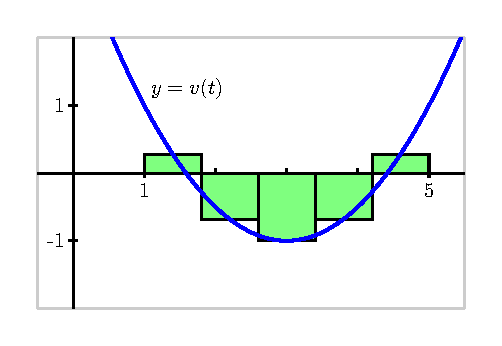
\includegraphics{figures/4_2_Act3Soln.eps}
	\end{center}
	\item Since the net signed area bounded by $v$ on $[1,5]$ represents the total change in position of the object on the interval $[1,5]$, it follows that $M_5$ estimates the total change in position.  Hence, the change in position is approximately $-1.44$ feet.
	\item To estimate the total distance traveled by the object on $[1,5]$, we have to calculate the total area between the curve and the $t$-axis.  Thus,
	$$D \approx \frac{7}{25} \cdot \frac{4}{5} + \frac{17}{25} \cdot \frac{4}{5} + 1 \cdot \frac{4}{5} + \frac{17}{25} \cdot \frac{4}{5} +  \frac{7}{25} \cdot \frac{4}{5} = \frac{292}{125} \approx 2.336.$$
	\item Using appropriate technology, $M_{10} = -1.36$ and $M_{20} = -1.34$.  Further calculations suggest that $M_n \to -\frac{4}{3} = -1.\overline{33}$ as $n \to \infty$, and this number represents the object's total change in position on $[1,5]$.
\ea
\end{activitySolution}
\aftera





